\section{Benutzeroberfläche}
%[TODO: remove this link] https://tex.stackexchange.com/questions/442077/is-it-possible-to-use-svg-images-with-overleaf

Bei den Abbildungen handelt sich hier lediglich um Entwürfe des Web-Interfaces. Dementsprechend sind Änderungen im Design vorbehalten. Das finale Produkt kann also von diesen Entwürfen abweichen.\\
Man beachte, das in den Entwürfen auch Funktionalität zu sehen ist, welche aus Wunschkriterien stammen. Diese sind hier nicht gesondert markiert oder hervorgehoben. Die auf diesen Entwürfen enthaltenen Markierungen (Kreise mit Zahlen und rotem Rand) dienen lediglich zur Lokalisierung der Erläuterungen und werden nicht im finalen Produkt enthalten sein.
\subsection{Anmeldung}
\label{pages:login}
\begin{figure}[H]
    \centering
    \includegraphics[width=\textwidth]{images-interface/v4_interface/login_page_4.pdf}
    \caption{Anmeldung}
    \label{fig:login}
\end{figure}
Auf dieser Seite kann sich ein \gls{Nutzer} mit einem bereits vorhandenen \gls{Nutzerkonto} anmelden. Diese Seite wird einem nicht angemeldetem \gls{Nutzer} standardmäßig bei Aufruf des \gls{Web-Interface} angezeigt. Ist ein \gls{Nutzer} bereits angemeldet, so wird er zur \hyperref[pages:job-table]{Job-Tabelle} weitergeleitet.\\
\newpage
\textbf{Erläuterungen}
\begin{itemize}
    \item[1)] Die Schaltfläche \enquote{Register} leitet zur \hyperref[pages:register]{Registrierungsseite} weiter.
    \item[2)] Die Schaltfläche \enquote{Log in} meldet den \gls{Nutzer} bei korrekt eingegebenen Daten an und leitet ihn zur \hyperref[pages:job-table]{Job-Tabelle} weiter.
\end{itemize}

\subsection{(Wunschkriterium) Registrierung}
\label{pages:register}
\begin{figure}[H]
    \centering
    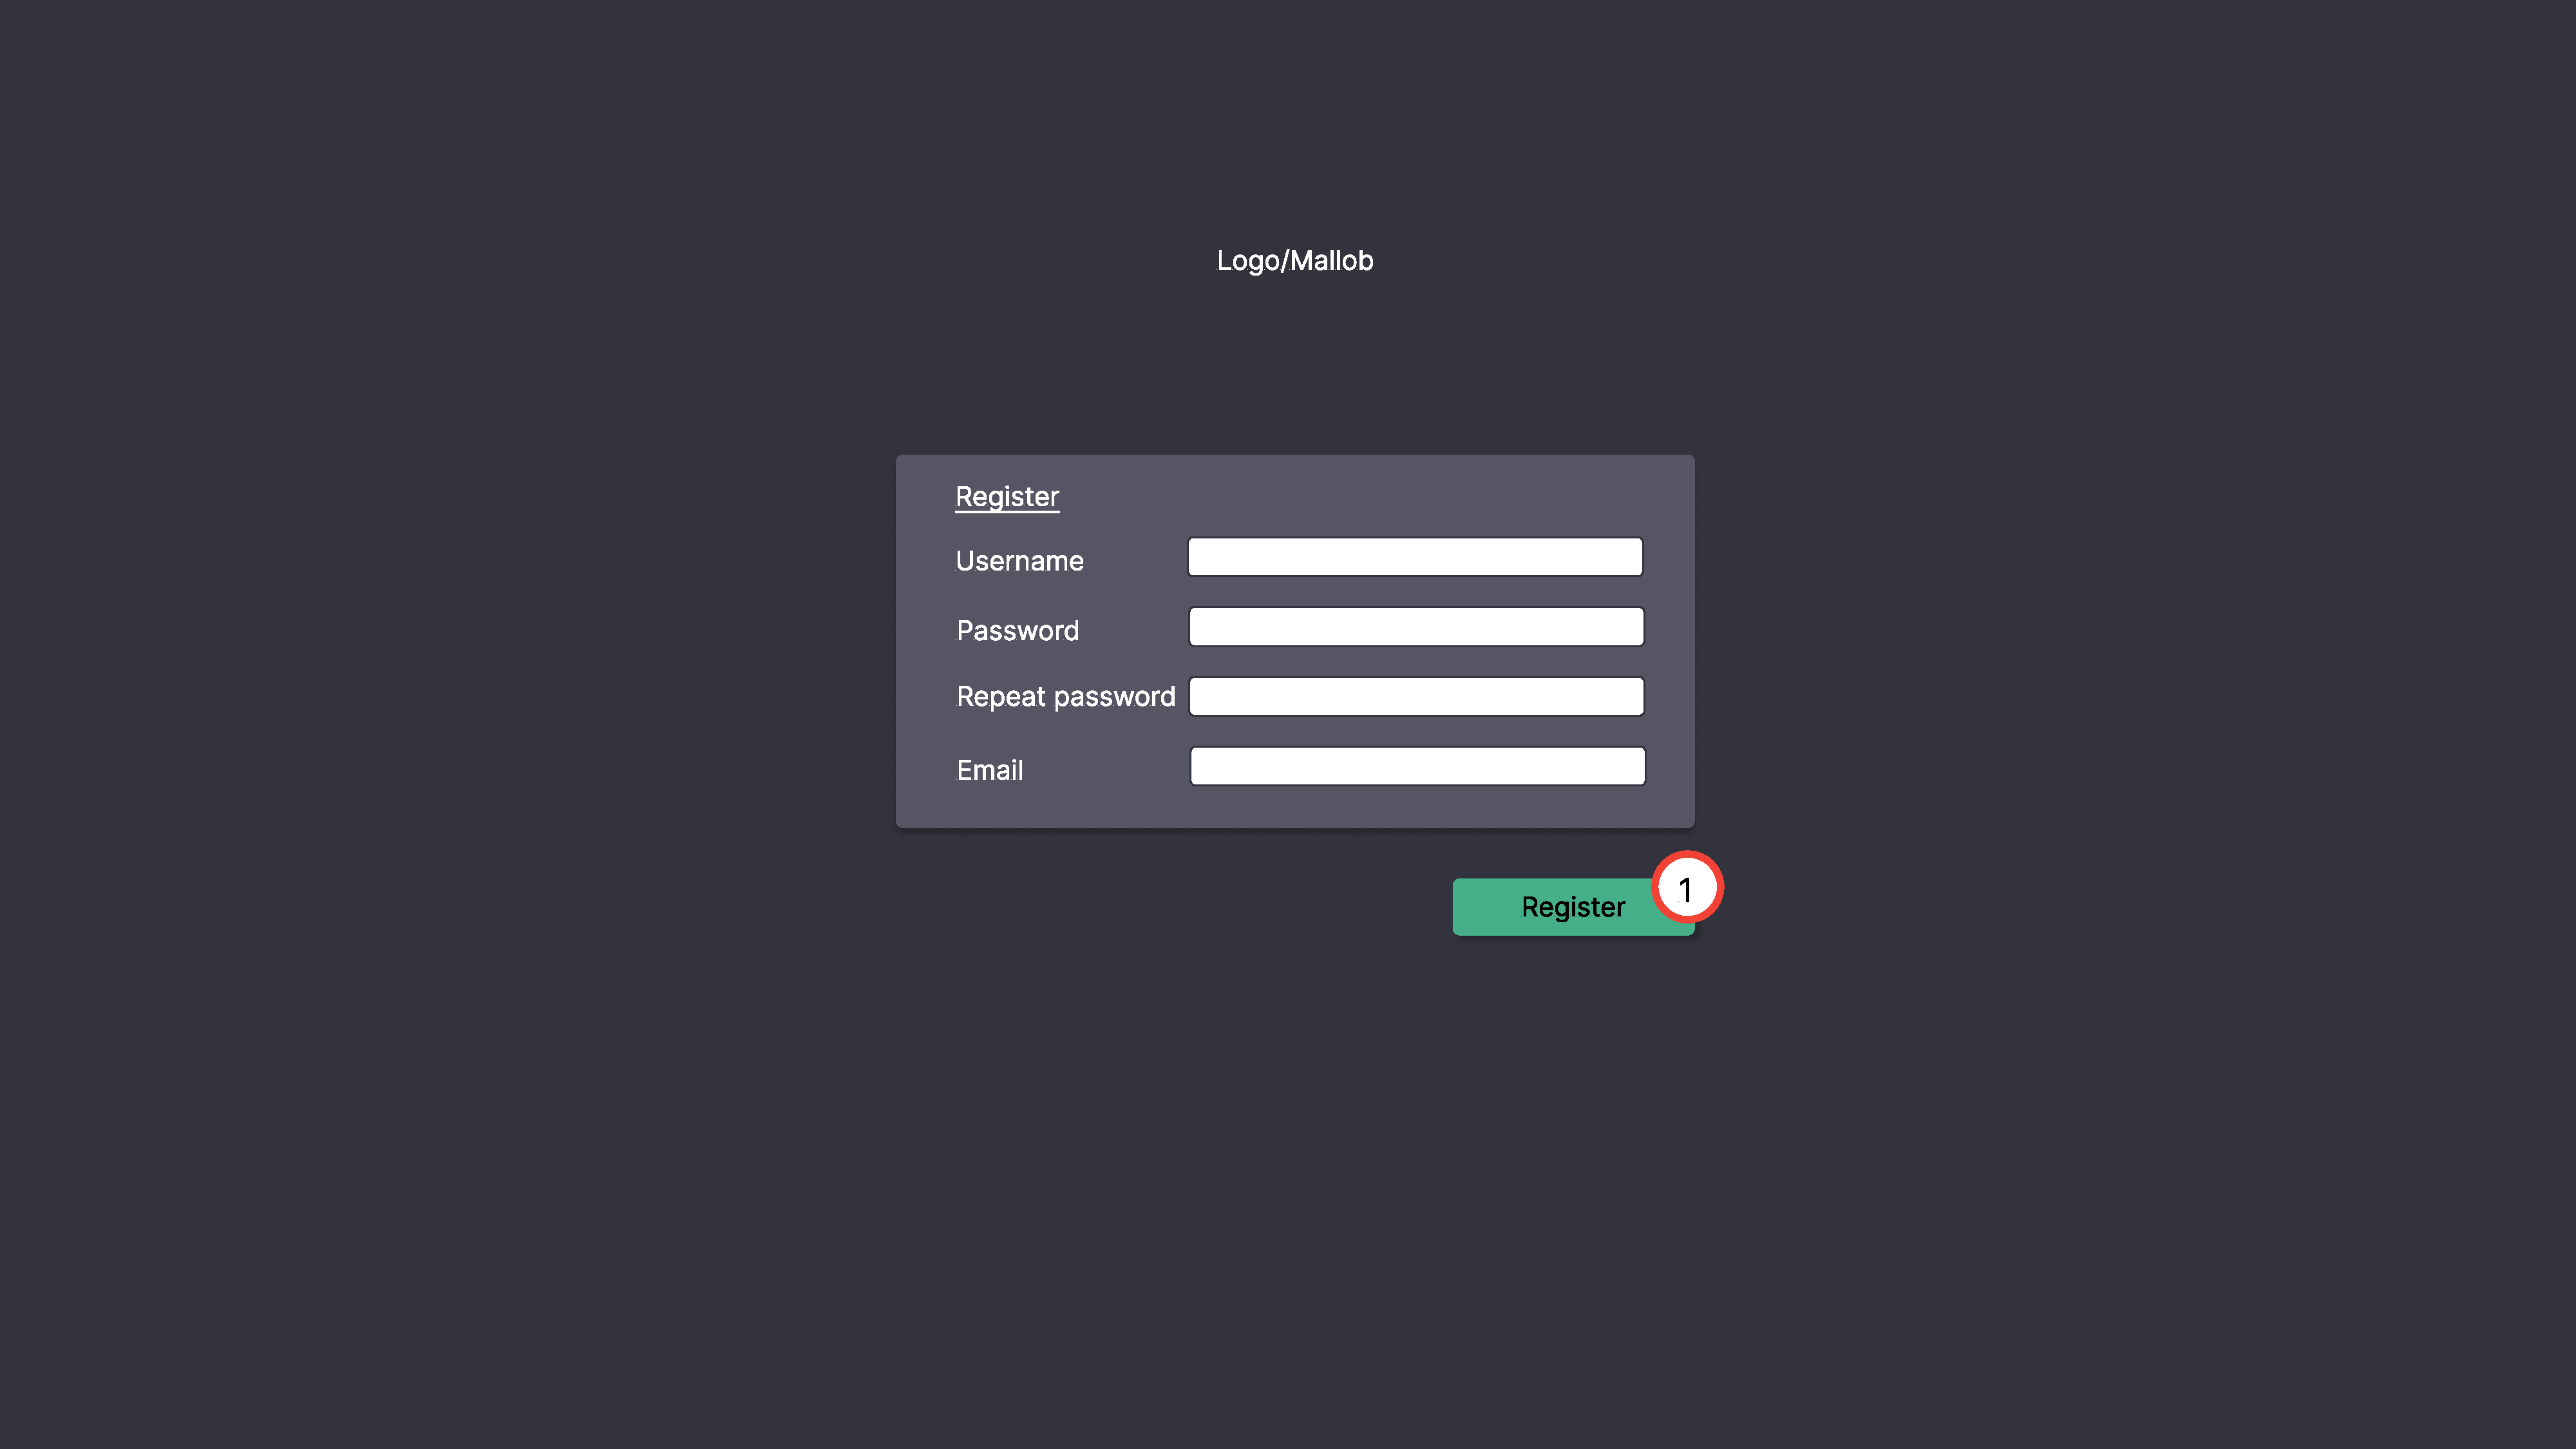
\includegraphics[width=\textwidth]{images-interface/v4_interface/register_page_4.pdf}
    \caption{Registrierung}
    \label{fig:register}
\end{figure}
Auf dieser Seite kann sich eine Person gemäß \hyperref[FA:Web-Interface:Registrierung von Nutzern]{F2120} registrieren. Sind die \hyperref[PD:Registrierungsdaten]{Eingabedaten} korrekt, wird ein neues vorläufiges \gls{Nutzerkonto} mit den entsprechenden Daten erstellt. \\


\textbf{Erläuterungen}
\begin{itemize}
    \item[1)] Die Schaltfläche \enquote{Register} registriert den \gls{Nutzer} und leitet ihn zur \hyperref[pages:visualization]{Visualisierung} weiter, da sein \gls{Nutzerkonto} direkt nach der Registrierung noch nicht verifiziert ist und er somit ohnehin noch keine \hyperref[B:Jobs]{Jobs} einreichen kann.
\end{itemize}



\newpage
\subsection{Job-Tabelle}
\label{pages:job-table}
Auf dieser Seite gibt es eine Übersicht über die \hyperref[B:Jobs]{Jobs}, die der \gls{Nutzer} bereits eingereicht hat. Das ganze findet in tabellarischer Form statt. Die Spalten \hyperref[B:Job-ID]{Job-ID} und \hyperref[B:Job-Status]{Job-Status} sowie die Spalte mit den \glspl{Checkbox} werden immer dargestellt, die restlichen Spalten sind alle optional auswählbar.\\

\subsubsection{Standard-Ansicht}
\label{pages:job-table-default}
\begin{figure}[H]
    \centering
    \label{fig:job-table-default}
    \includegraphics[width=\textwidth]{images-interface/v6_interface/job_table_split_6.pdf}
    \caption{Standard-Ansicht der Job-Tabelle}
\end{figure}

In dieser Standard-Ansicht lassen sich durch anklicken eines \hyperref[B:Jobs]{Jobs} in der Tabelle Informationen zu diesem im nebenstehenden Fenster anzeigen.
Der Inhalt des nebenstehenden Fensters stimmt mit dem der \hyperref[pages:job-page]{Job-Seite} überein.\\

\textbf{Erläuterungen}
\begin{itemize}
    \item[1)] Über dieses \gls{Dropdown-Menue} kann die Ansicht der Tabelle gewechselt werden. Standardmäßig wird die Standard-Ansicht angezeigt.
    \item[2)] Über diese Schaltfläche kann das Ergebnis gemäß \hyperref[FA:Web-Interface:Herunterladen eines einzelnen Ergebnisses]{F2040} heruntergeladen werden. Man beachte, dass diese Schaltfläche nur bei abgeschlossenen \hyperref[B:Jobs]{Jobs} verfügbar ist. Bei laufenden \hyperref[B:Jobs]{Jobs} bietet sie die Möglichkeit, den \hyperref[B:Jobs]{Job} gemäß \hyperref[FA:Web-Interface:Abbruch eines einzelnen Jobs]{F2020} abzubrechen. Bei abgebrochenen \hyperref[B:Jobs]{Jobs} bietet sie die Möglichkeit, den \hyperref[B:Jobs]{Job} gemäß \hyperref[Neustart eines abgebrochenen Jobs]{F2130} neuzustarten.
   \item[3)] Über diese Schaltfläche wird der \gls{Nutzer} zur entsprechenden \hyperref[pages:job-page]{Job-Seite} des \hyperref[B:Jobs]{Jobs} weitergeleitet.
\end{itemize}

%\textbf{Erläuterungen}
%\begin{itemize}
%    \item[1)] Über dieses \gls{Dropdown-Menue} kann die Ansicht der Tabelle gewechselt werden. Standardmäßig wird die Standard-Ansicht angezeigt.
%    \item[2)] Über dieses \gls{Dropdown-Menue} können gemäß \hyperref[FA:Web-Interface:Hinzufügen von Spalten]{F2090} weitere Attribute in der Tabelle angezeigt werden.
%    \item[3)] Über diese \gls{Checkbox} kann gemäß \hyperref[FA:Web-Interface:Filtern für Admins]{F2160} ausgewählt werden, ob in der Tabelle alle Jobs oder nur die Jobs des angemeldeten Nutzers zu sehen sind. Ist nur für Administratoren verfügbar.
%    \item[4)] Über diese Schaltfläche kann die Job-Tabelle gemäß \hyperref[Aktualisieren der Job-Tabelle]{F2105} aktualisiert werden.
%    \item[5)] Über dieses \gls{Dropdown-Menue} kann eine Aktion (siehe \hyperref[FA:Web-Interface:Abbruch mehrerer Jobs auf einmal]{F2030} und \hyperref[FA:Web-Interface:herunterladen mehrerer Ergebnisse auf einmal]{FA2050}) durchgeführt werden, welche auf alle mit der \gls{Checkbox} ausgewählten \hyperref[B:Jobs]{Jobs} angewandt wird.
%    \item[6)] Über das Symbol mit den beiden Dreiecken kann die entsprechende Spalte gemäß \hyperref[FA:Web-Interface:Sortieren der Tabelle]{F2150} sortiert werden. Mit dem Kreuz-Symbol kann die Spalte gemäß \hyperref[FA:Web-Interface:Entfernen von Spalten]{F2100} wieder aus der Tabelle gelöscht werden.
%    \item[7)] Über diese \glspl{Checkbox} kann ein \hyperref[B:Jobs]{Job} für eine Aktion nach Punkt Zwei dieser Liste ausgewählt werden.
%    \item[8)] Über diese Schaltfläche kann das Ergebnis gemäß \hyperref[FA:Web-Interface:Herunterladen eines einzelnen Ergebnisses]{F2040} heruntergeladen werden. Man beachte, dass diese Schaltfläche nur bei abgeschlossenen \hyperref[B:Jobs]{Jobs} verfügbar ist. Bei laufenden \hyperref[B:Jobs]{Jobs} bietet sie die Möglichkeit, den \hyperref[B:Jobs]{Job} gemäß \hyperref[FA:Web-Interface:Abbruch eines einzelnen Jobs]{F2020} abzubrechen. Bei abgebrochenen \hyperref[B:Jobs]{Jobs} bietet sie die Möglichkeit, den \hyperref[B:Jobs]{Job} gemäß \hyperref[Neustart eines abgebrochenen Jobs]{F2130} neuzustarten.
%    \item[9)] Über diese Schaltfläche wird der \gls{Nutzer} zur entsprechenden \hyperref[pages:job-page]{Job-Seite} des \hyperref[B:Jobs]{Jobs} weitergeleitet.
%\end{itemize}
\newpage
\subsubsection{(Wunschkriterium) Alternative Ansicht}
\begin{figure}[H]
    \label{fig:job-table-exp}
    \includegraphics[width=\textwidth]{images-interface/v5_interface/job_table_expanded_5.pdf}
    \caption{Alternative Ansicht der Job-Tabelle}
\end{figure}
Bei dieser alternativen Ansicht der \hyperref[pages:job-table]{Job-Tabelle} werden beim Ankicken eines \hyperref[B:Jobs]{Jobs} die Informationen in einem aufgeklapptem Fenster unterhalb der Zeile des angeklickten \hyperref[B:Jobs]{Jobs} angezeigt. Der Informationsgehalt und die Funktionalität dieser Ansicht ist identisch mit der der \hyperref[pages:job-table-default]{Standard-Ansicht}. \\
Diese alternative Ansicht kann somit auch immer genutzt werden, wenn die \hyperref[pages:job-table]{Job-Tabelle} referenziert wird, nur eben mit dem Unterschied, das die Information eines angeklickten \hyperref[B:Jobs]{Jobs} im aufgeklappten Fenster angezeigt werden.
Zu jedem Zeitpunkt ist immer nur maximal ein \hyperref[B:Jobs]{Job} aufgeklappt. Sollte bereits ein \hyperref[B:Jobs]{Job} aufgeklappt sein, so wird er wieder eingeklappt, wenn ein anderer aufgeklappt wird.\\



\newpage
\subsection{Job einreichen}
\label{pages:submit-job}
\begin{figure}[H]
    \centering
    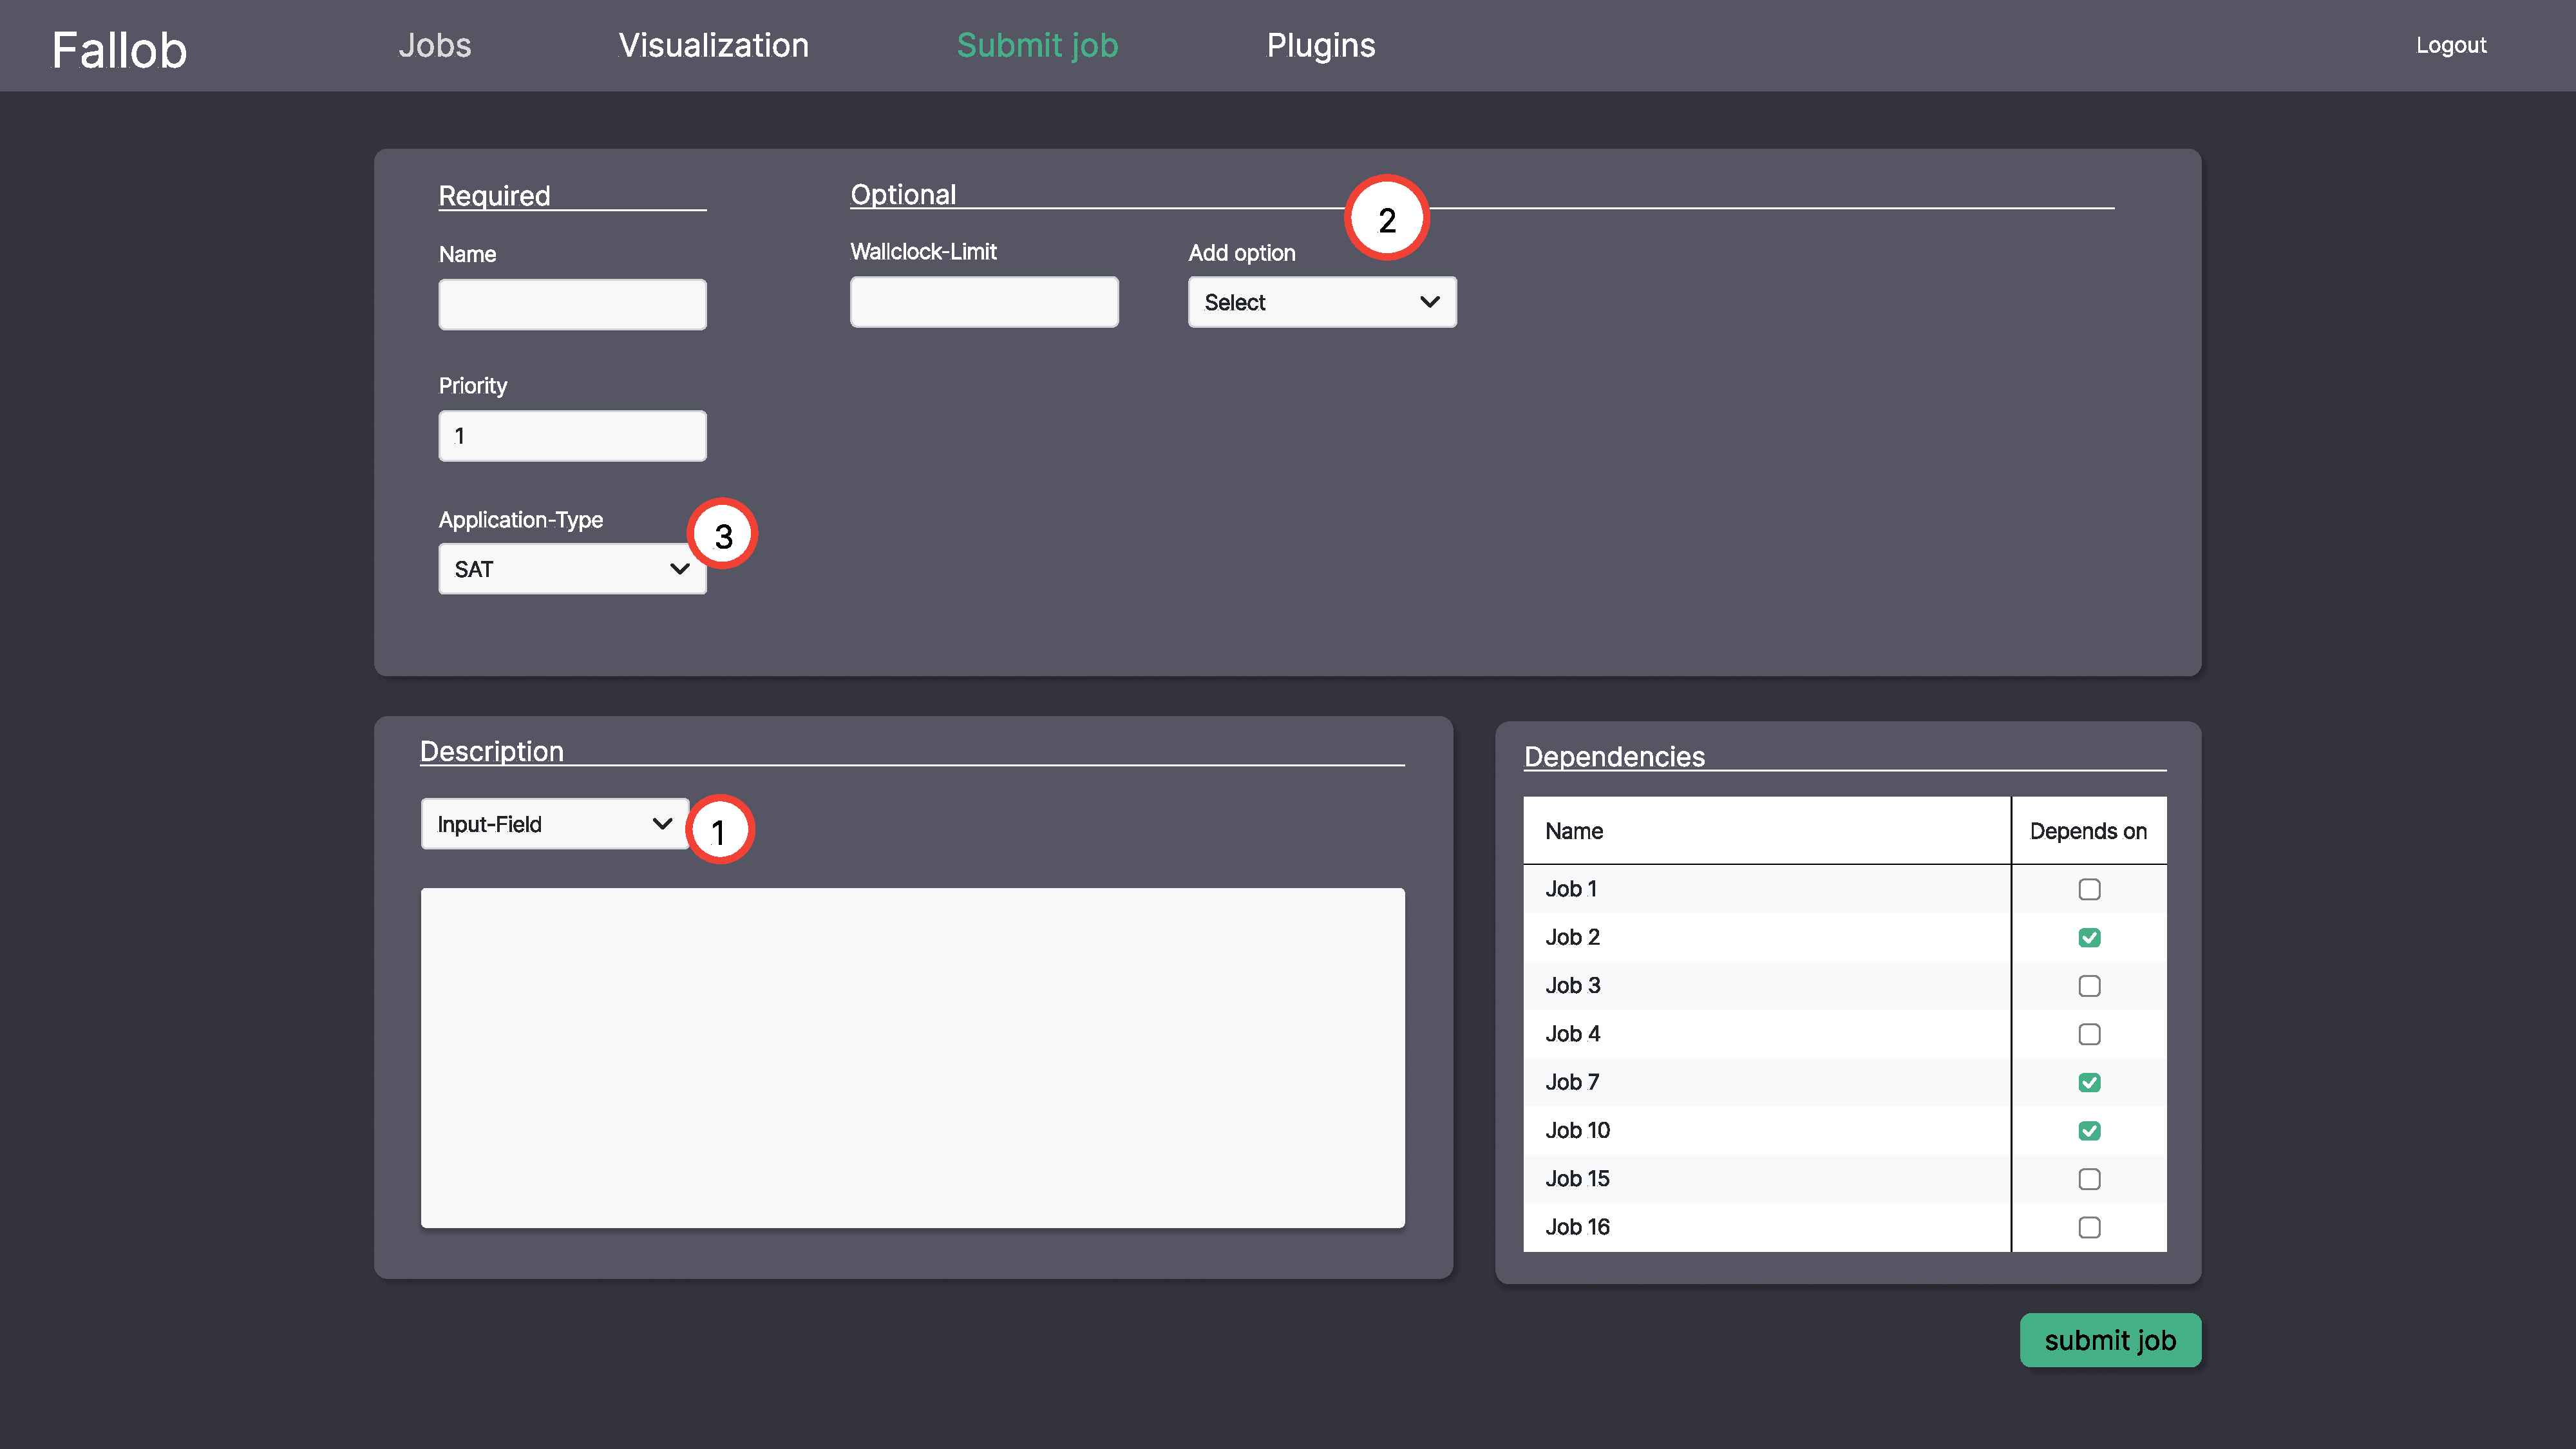
\includegraphics[width=\textwidth]{images-interface/v4_interface/submit_job_page_4.pdf}
    \caption{Einreichen neuer \hyperref[B:Jobs]{Jobs}}
    \label{fig:submit-job}
\end{figure}
Auf dieser Seite können neue \hyperref[B:Jobs]{Jobs} eingereicht werden. Es gibt die Möglichkeit, die \hyperref[B:Job-Konfiguration]{Job-Konfiguration} korrekt einzustellen, die \hyperref[B:Job-Beschreibung]{Job-Beschreibung} hinzuzufügen sowie die Möglichkeit, Abhängigkeiten zu anderen \hyperref[B:Jobs]{Jobs} anzugeben. \\

\textbf{Erläuterungen}
\begin{itemize}
    \item[1)] Mit diesem \gls{Dropdown-Menue} kann gemäß \hyperref[FA:Web-Interface:Job einreichen]{F2010} gewählt werden, auf welchem Wege die \hyperref[B:Job-Beschreibung]{Job-Beschreibung} übermittelt wird. Die \hyperref[B:Job-Beschreibung]{Job-Beschreibung} muss auf genau einem dieser Wege übermittelt werden.
    \item[2)] Mit diesem \gls{Dropdown-Menue} können weitere, optionale Job-Parameter gemäß \hyperref[FA:Web-Interface:Job einreichen]{F2010} ausgewählt werden. 
    \item[3)] Mit diesem \gls{Dropdown-Menue} kann der \hyperref[B:Job-Typ]{Job-Typ} ausgewählt werden. Zur Auswahl stehen \gls{SAT}, \hyperref[B:Job-Typ]{DUMMY} und \gls{k-Means}.
\end{itemize}

\newpage
\subsection{Job-Seite}
\label{pages:job-page}
\begin{figure}[H]
    \centering
    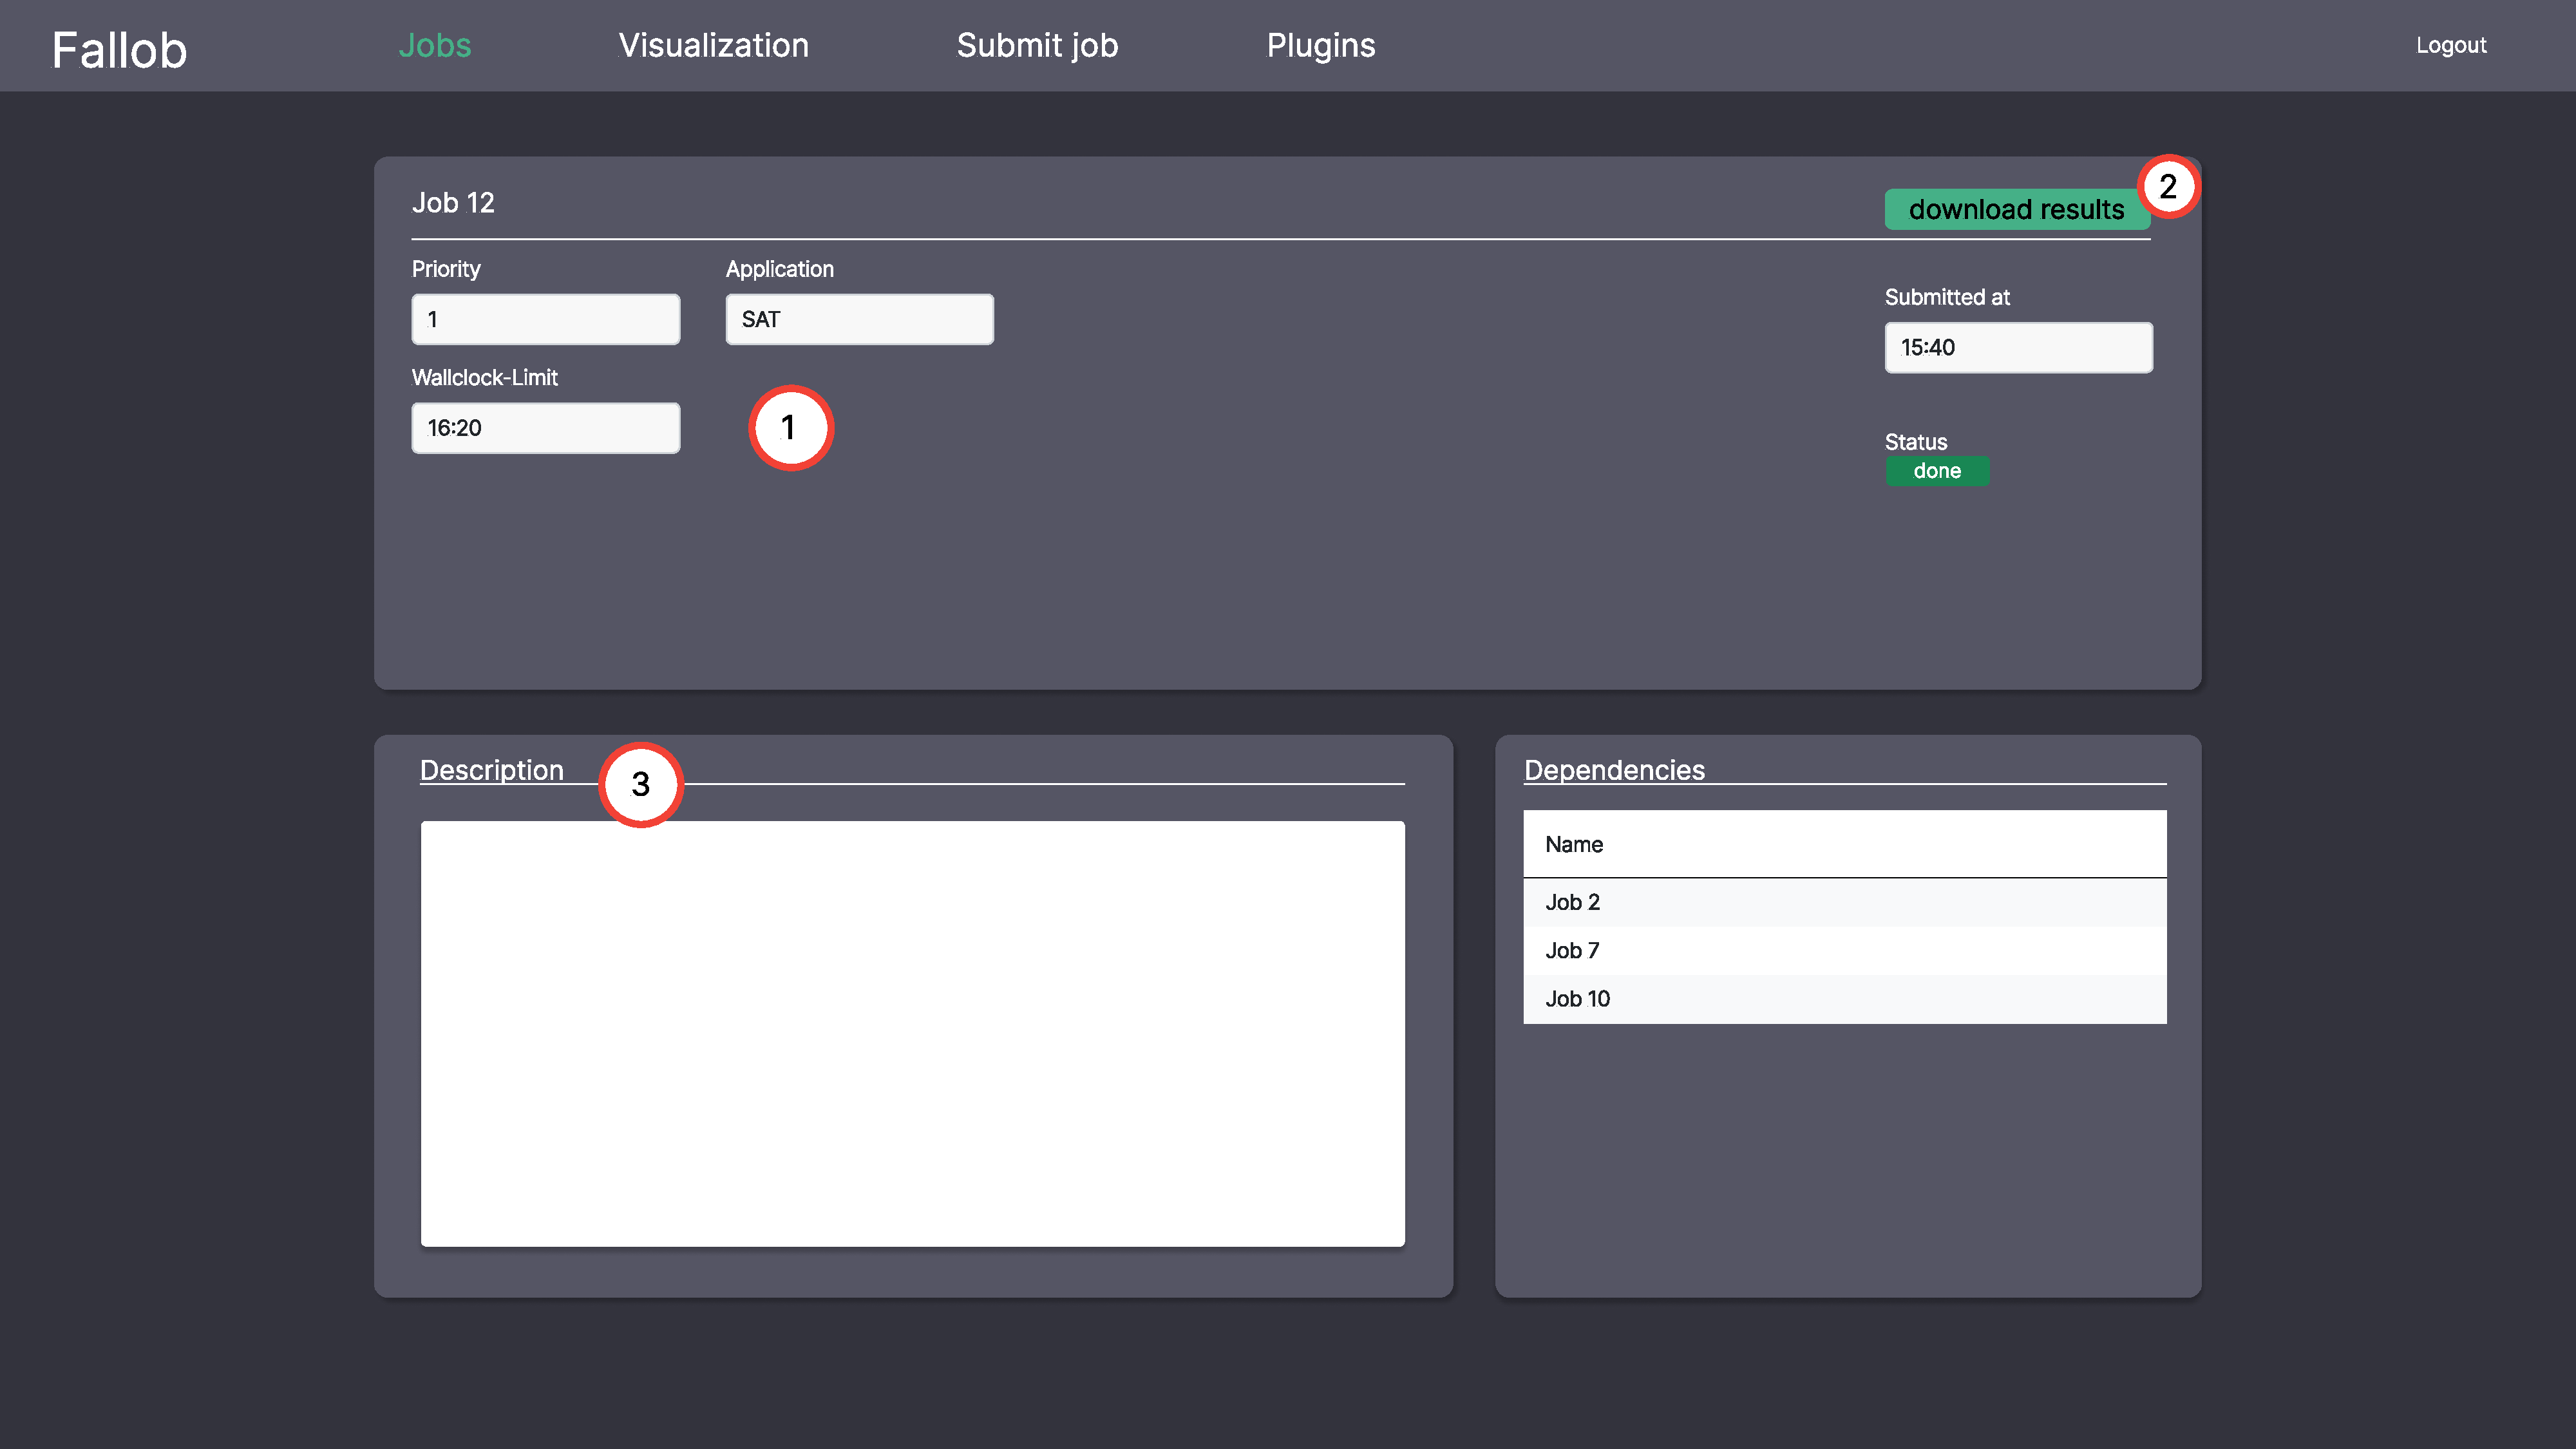
\includegraphics[width=\textwidth]{images-interface/v5_interface/job_info_page_5.pdf}
    \caption{Info-Seite eines \hyperref[B:Jobs]{Jobs}}
    \label{fig:job-page}
\end{figure}
Diese Seite bietet eine Übersicht über einen einzelnen \hyperref[B:Jobs]{Job}. Es werden die \hyperref[B:Job-Konfiguration]{Job-Konfiguration}, die \hyperref[B:Job-Beschreibung]{Job-Beschreibung}, die Abhängigkeiten, den Zeitpunkt des Einreichens und der aktuelle \hyperref[B:Job-Status]{Status} angezeigt. Weiterhin besteht die hier die Möglichkeit, das Ergebnis eines abgeschlossenen \hyperref[B:Jobs]{Jobs} herunterzuladen. Man gelangt zu dieser Seite gemäß \hyperref[FA:Web-Interface:Einsehen von Job-Informationen]{F2140}.

\textbf{Erläuterungen}
\begin{itemize}
    \item[1)] Hier werden möglicherweise auch noch weitere, für diesen \hyperref[B:Jobs]{Job} gewählten optionale Parameter angezeigt.
    \item[2)] Über diese Schaltfläche kann das Ergebnis gemäß \hyperref[FA:Web-Interface:Herunterladen eines einzelnen Ergebnisses]{F2040} heruntergeladen werden. Man beachte, dass diese Schaltfläche nur bei abgeschlossenen \hyperref[B:Jobs]{Jobs} verfügbar ist. Bei laufenden \hyperref[B:Jobs]{Jobs} bietet sie die Möglichkeit, den \hyperref[B:Jobs]{Job} gemäß \hyperref[FA:Web-Interface:Abbruch eines einzelnen Jobs]{F2020} abzubrechen. Bei abgebrochenen \hyperref[B:Jobs]{Jobs} bietet sie die Möglichkeit, den \hyperref[B:Jobs]{Job} gemäß \hyperref[Neustart eines abgebrochenen Jobs]{F2130} neuzustarten.
\end{itemize}

\newpage
\subsection{Visualisierung}
\label{pages:visualization}
\begin{figure}[H]
    \centering
    \includegraphics[width=\textwidth]{images-interface/v6_interface/visualization_page_6.pdf}
    \caption{Visualisierung des Systems}
    \label{fig:visualization-page}
\end{figure}
Diese Seite visualisiert den \gls{Systemzustand}. Im linken Fenster ist hierbei die Ansicht der \glspl{Prozess} und zugeordneten \hyperref[B:Jobs]{Jobs} zu sehen. Das Fenster rechts ist zunächst leer. Es wird, wie hier zu sehen, erst mit Informationen gefüllt, wenn der \gls{Nutzer} auf einen Prozess im Fenster links auswählt. Dann werden zu diesem einen Prozess der Rank, die Größe des \gls{Binaerbaum}, die Größe des ausgewählten \glslink{Teilbaum}{Teilbaumes} und Informationen über den \gls{Nutzer}.\\

\textbf{Erläuterungen}
\begin{itemize}
    \item[1)] Verwendet Mallob mehr \glspl{Prozess} als auf dieser Seite angezeigt werden können, so erscheint eine Scrollbar, mithilfe derer die Ansicht vertikal verschoben werden kann.
    \item[2)] Hier findet die eigentliche Visualisierung gemäß \hyperref[FA:Web-Interface:Verifizieren eines Kontos]{FA3000} statt. In diesem Falle ist ein \gls{Administrator} angemeldet (erkennbar daran, das Schaltfläche \enquote{Administration} in der Navigations-Leiste sichtbar ist), daher sind alle \hyperref[B:Jobs]{Jobs} farbig und nicht in Grautönen. Für einen nicht-\gls{Administrator} werden \hyperref[B:Jobs]{Jobs} von anderen Nutzern pseudonymisiert und grau angezeigt.
    \item[3)] Hier wird gemäß \hyperref[FA:Visualisierung:Anzeigen des Binaerbaumes für einen Job]{FA3010} der \gls{Binaerbaum} aus ausgewählten \hyperref[B:Jobs]{Jobs} angezeigt.
    \item[4)] Informationen über den \gls{Nutzer}, dem der \hyperref[B:Jobs]{Job} gehört. Wird nur angezeigt, da ein \gls{Administrator} angemeldet ist.
\end{itemize}

%Anmerkung zur Plugin einsicht; Evtl oben in der Querleiste ein Reiter "Plugins" und das dann als Dropdown menü für alle hinzugefügtten Plugins machen. Das macht die Seite stabiler für viele Plguins
% gute idee, schaff ich heute aber nicht mehr

\subsection{(Wunschkriterium) Plugin-Ansicht}
\label{pages:plugin}
\begin{figure}[H]
    \centering
    \includegraphics[width=\textwidth]{images-interface/v4_interface/plugin_page_4.pdf}
    \caption{Generische Ansicht für \glspl{Plugin}}
    \label{fig:plugin-page}
\end{figure}
Diese Seite stellt die generische Ansicht für \glspl{Plugin} dar. Um zu dieser Seite zu gelangen, kann man oben über das \gls{Dropdown-Menue} in der Navigations-Leiste ein verfügbares \gls{Plugin} auswählen. Gibt es keine \glspl{Plugin}, so wird das \gls{Dropdown-Menue} nicht angezeigt. \\

\textbf{Erläuterungen}
\begin{itemize}
    \item[1)] Hier kann der \hyperref[B:Jobs]{Job} ausgewählt werden, welcher vom \gls{Plugin} verarbeitet wird.
    \item[2)] Diese Fläche steht dem \gls{Plugin} frei zur Darstellung zur Verfügung.
\end{itemize}

\newpage
\subsection{Administration}
\label{pages:admin}
\begin{figure}[H]
    \centering
    \includegraphics[width=\textwidth]{images-interface/v4_interface/admin_page_4.pdf}
    \caption{Seite für \glspl{Administrator} zur Verwaltung des Systems}
    \label{fig:admin-page}
\end{figure}
Diese Seite dient der Verwaltung des Systems. Sie ist nur für angemeldete \glspl{Administrator} sichtbar. \\

\textbf{Erläuterungen}
\begin{itemize}
    \item[1)] Hier wird kann die Instanz von Mallob verwaltet.
    \item[2)] Hier werden gemäß \hyperref[FA:Web-Interface:Anzeigen von Warungen und Fehlermeldungen]{FA2110} Warnungen und Fehlermeldungen angezeigt, die Mallob ausgibt.
    \item[3)] Hier werden gemäß \hyperref[]{[TODO]} Diagnose-Daten angezeigt.
\end{itemize}

%\newpage
%\subsection{Funktionen}
%\begin{itemize}
%    \item /B010/ Es sind zwei Sichten zu unterscheiden: die des Admins, die des Benutzers. 
%    \item /B020/ Benutzer können Funktionen F10, F20, F30 jederzeit nach dem Einloggen aufrufen.
%    \item /B030/ Jeder Benutzer fängt auf der Login/Register-Seite an.
%    \item /B040/ Sobald der Benutzer eingeloggt wird, sieht er die Startseite.
%    \item /B050/ Jeder \gls{Nutzer} kann seine \hyperref[B:Jobs]{Jobs} anhand der Aufwand auf das Kern unterscheiden (z.B Farbe, Größe usw.)
%    \item /B060/ Admins können alle Funktionen, die die Benutzer können.
%    \item /B070/ Unterschiedliche Benutzer und ihre Befugnisse sollen entsprechend behandelt werden (nicht-funktionale Anforderung?).
%    \item /B080/ Die Bedienungsoberfläche ist auf Mausbedienung auszulegen; eine Bedienung ohne Maus muss aber auch möglich sein. ([TODO] Bediengung ohne Maus auf jeden Fall wunschkriterium oder vlt sogar gar nicth, auf jeden Fall mal fragen, hört sich kompliziert und nicht wirklich notwendig an)
%\end{itemize}